\documentclass[11pt]{article}

\usepackage[letterpaper,margin=0.75in]{geometry}
\usepackage{booktabs}
\usepackage{caption}
\usepackage{graphicx}
\usepackage{listings}
\usepackage{float}
\usepackage{scrextend}

\usepackage[parfill]{parskip}
\renewcommand{\lstlistingname}{Snippet}


\begin{document}

\lstset{
  language=Python,
  basicstyle=\small,          % print whole listing small
  keywordstyle=\bfseries,
  identifierstyle=,           % nothing happens
  commentstyle=,              % white comments
  stringstyle=\ttfamily,      % typewriter type for strings
  showstringspaces=false,     % no special string spaces
  numbers=left,
  numberstyle=\tiny,
  numbersep=5pt,
  frame=tb,
}

\title{Network Simulation}

\author{Brandt Elison & Joe Eklund}

\date{January 26, 2016}

\maketitle

\section{Two Nodes}

The following experiments were performed on a simulated two-node network with two unidirection links connecting each node to the other. Throughout the rest of this section, we will refer to these two nodes as $n_1$ and $n_2$.

This section details three experiments done with this network. Each experiment measures the delay on one or more packets being sent from $n_1$ to $n_2$. The experiments each use different values for link speed, propagation delay, and the number and timing of packets sent. The simulated packets in these experiments are all of size 1000 bytes.

\begin{description}
\item[Experiment 1] \hfill \break
The following parameters were used for this experiment:

\begin{itemize}
\item Link speed: 1 Mbps
\item Propagation delay: 1000 ms
\item Packets sent: 1 packet at $t = 0$
\end{itemize}

\medskip

Snippet \ref{sec1exp1} below was used to create the network.

\medskip

\begin{lstlisting}[caption={Network 1.1},label=sec1exp1]
# The 'path' variable below references the following network configuration:
# n1 n2
# n2 n1
## link configuration
# n1 n2 1Mbps 1000ms
# n2 n1 1Mbps 1000ms

# setup network
net = Network(path)

# setup routes
n1 = net.get_node('n1')
n2 = net.get_node('n2')
n1.add_forwarding_entry(address=n2.get_address('n1'),link=n1.links[0])
n2.add_forwarding_entry(address=n1.get_address('n2'),link=n2.links[0])

# setup app
d = DelayHandler()
net.nodes['n2'].add_protocol(protocol="delay",handler=d)

p = packet.Packet(destination_address=n2.get_address('n1'),ident=1, \
                  protocol='delay',length=1000)
Sim.scheduler.add(delay=0, event=p, handler=n1.send_packet)
\end{lstlisting}

The following calculations show that the expected delay for this simulation should be 1.008 seconds:
\begin{addmargin}[1em]{0em}
$delay_{trans} = \frac{8000 bits}{10^{6}bps} = 0.008s = 8ms$

$delay_{prop} = 1000ms$

$delay_{total} = delay_{trans} + delay_{prop} = 1008ms = 1.008s$
\end{addmargin}

\bigskip

The simulator output is shown in Table \ref{tbl1.1}:

\smallskip

\begin{table}[H]
\begin{center}
\caption{Simulator output for Network 1.1}
\label{tbl1.1}
\begin{tabular}{ccccc}
  \toprule
  Arrival Time & Created Time & Transmission Delay & Propagation Delay & Queueing Delay\\
  \midrule
  1.008 & 0 & 0.008 & 1.0 & 0\\
  \bottomrule
\end{tabular}
\end{center}
\end{table}

\smallskip

The Arrival Time in Table \ref{tbl1.1} represents the total delay from transmitting the packet. This value for delay (1.008 seconds) matches the delay that we calculated by hand, which shows that the simulator is accurate.

\item[Experiment 2] \hfill \break
The following parameters were used for this experiment:

\begin{itemize}
\item Link speed: 100 bps
\item Propagation delay: 10 ms
\item Packets sent: 1 packet at $t = 0$
\end{itemize}

\medskip

Snippet \ref{sec1exp2} was used to create the network.

\medskip

\begin{lstlisting}[caption={Network 1.2},label=sec1exp2]
# The 'path' variable below references the following network configuration:
# n1 n2
# n2 n1
## link configuration
# n1 n2 100bps 10ms
# n2 n1 100bps 10ms

# setup network
net = Network(path)

# setup routes
n1 = net.get_node('n1')
n2 = net.get_node('n2')
n1.add_forwarding_entry(address=n2.get_address('n1'),link=n1.links[0])
n2.add_forwarding_entry(address=n1.get_address('n2'),link=n2.links[0])

# setup app
d = DelayHandler()
net.nodes['n2'].add_protocol(protocol="delay",handler=d)

p = packet.Packet(destination_address=n2.get_address('n1'),ident=1, \
                  protocol='delay',length=1000)
Sim.scheduler.add(delay=0, event=p, handler=n1.send_packet)
\end{lstlisting}

The following calculations show that the expected delay for this simulation should be 80.01 seconds:
\begin{addmargin}[1em]{0em}
$delay_{trans} = \frac{8000 bits}{100 bps} = 80s $

$delay_{prop} = 10ms = 0.01s$

$delay_{total} = delay_{trans} + delay_{prop} = 80.01s $
\end{addmargin}

\bigskip

The simulator output is shown in Table \ref{tbl1.2}:

\smallskip

\begin{table}[H]
\begin{center}
\caption{Simulator output for Network 1.2}
\label{tbl1.2}
\begin{tabular}{ccccc}
  \toprule
  Arrival Time & Created Time & Transmission Delay & Propagation Delay & Queueing Delay\\
  \midrule
  80.01 & 0 & 80.0 & 0.01 & 0\\
  \bottomrule
\end{tabular}
\end{center}
\end{table}

\smallskip

The Arrival Time in Table \ref{tbl1.2} represents the total delay from transmitting the packet. This value for delay (80.01 seconds) matches the delay that we calculated by hand, which shows that the simulator is accurate.

\item[Experiment 3] \hfill \break
The following parameters were used for this experiment:

\begin{itemize}
\item Link speed: 1 Mbps
\item Propagation delay: 10 ms
\item Packets sent: 3 packets at $t = 0$; 1 packet at $t = 2s$. We will refer to these packets as $p_1$, $p_2$, $p_3$, and $p_4$ respectively
\end{itemize}

\medskip

Snippet \ref{sec1exp3} was used to create the network.

\medskip

\begin{lstlisting}[caption={Network 1.3},label=sec1exp3]
# The 'path' variable below references the following network configuration:
# n1 n2
# n2 n1
## link configuration
# n1 n2 1Mbps 10ms
# n2 n1 1Mbps 10ms

# setup network
net = Network(path)

# setup routes
n1 = net.get_node('n1')
n2 = net.get_node('n2')
n1.add_forwarding_entry(address=n2.get_address('n1'),link=n1.links[0])
n2.add_forwarding_entry(address=n1.get_address('n2'),link=n2.links[0])

# setup app
d = DelayHandler()
net.nodes['n2'].add_protocol(protocol="delay",handler=d)

p1 = packet.Packet(destination_address=n2.get_address('n1'),ident=1, \
                    protocol='delay',length=1000)
Sim.scheduler.add(delay=0, event=p1, handler=n1.send_packet)

p2 = packet.Packet(destination_address=n2.get_address('n1'),ident=1, \
                    protocol='delay',length=1000)
Sim.scheduler.add(delay=0, event=p2, handler=n1.send_packet)

p3 = packet.Packet(destination_address=n2.get_address('n1'),ident=1, \
                    protocol='delay',length=1000)
Sim.scheduler.add(delay=0, event=p3, handler=n1.send_packet)

# Late packet
p4 = packet.Packet(destination_address=n2.get_address('n1'),ident=1, \
                    protocol='delay',length=1000)
Sim.scheduler.add(delay=2, event=p4, handler=n1.send_packet)
\end{lstlisting}

The following calculations show the expected delay for $p_1$:
\begin{addmargin}[1em]{0em}
$delay_{trans} = \frac{8000 bits}{10^{6}bps} = 0.008s = 8ms$

$delay_{prop} = 10ms = 0.01s$

$delay_{total} = delay_{trans} + delay_{prop} = 0.018s $
\end{addmargin}

$p_2$, $p_3$, and $p_4$ are the same size as $p_1$, so each takes the same amount of time to go from $n_1$ to $n_2$ once they have begun to transmit. However, $p_2$, $p_3$, and $p_4$ have extra delay for various reasons, so they do not arrive at $t = .018s$ like $p_1$ does.

$p_2$ and $p_3$ are delayed by queing delay as they wait for their turn to begin transmitting. Each must wait for the transmission delay of the previous packet(s) to elapse before it can begin to transmit, so the following delays exist for $p_2$ and $p_3$:
\begin{addmargin}[1em]{0em}
$delay_{p_{2}} = delay_{p_{1}} + delay_{trans} = 0.026s$

$delay_{p_{3}} = delay_{p_{2}} + delay_{trans} = 0.034s$
\end{addmargin}

$p_4$ is delayed purely because it is transmitted 2 seconds later than the other packets. By the time it begins transmitting, the other packets have already arrived at $n_2$. Therefore,
\begin{addmargin}[1em]{0em}
$delay_{p_{4}} = 2s + delay_{p_{1}} = 2.018s$
\end{addmargin}

\medskip

The simulator output is shown in Table \ref{tbl1.3}.

\smallskip

\begin{table}[H]
\begin{center}
\caption{Simulator output for Network 1.3}
\label{tbl1.3}
\begin{tabular}{cccccc}
  \toprule
  Packet & Arrival Time & Created Time & Transmission Delay & Propagation Delay & Queueing Delay\\
  \midrule
  $p1$ & 0.018 & 0 & 0.008 & 0.01 & 0\\
  $p2$ & 0.026 & 0 & 0.008 & 0.01 & 0.008\\
  $p3$ & 0.034 & 0 & 0.008 & 0.01 & 0.016\\
  $p4$ & 2.018 & 2.0 & 0.008 & 0.01 & 0.0\\
  \bottomrule
\end{tabular}
\end{center}
\end{table}

\smallskip

The Arrival Time in Table \ref{tbl1.3} represents the total delay from transmitting each packet in order. The values for delay (.018, .026, .034, and 2.018 seconds) match the delay that we calculated by hand, which shows that the simulator is accurate. We can also see in Table \ref{tbl1.3} that $p_2$ and $p_3$ experienced queueing delay as expected.

\end{description}

\section{Three Nodes}

The following experiments were performed on a simulated three-node network with two unidirection links connecting $n_1$ with $n_2$ and two unidirection links connecting $n_2$ with $n_3$. Throughout the rest of this section, we will refer to these three nodes as $n_1$, $n_2$, and $n_3$.

This section details two experiments done with this network. Each experiment measures the delay on one or more packets being sent from $n_1$ to $n_3$. The experiments each use different values for link speeds and propagation delays. The simulated packets in these experiments are all of size 1000 bytes.

\begin{description}
\item[Experiment 1] \hfill \break
The following parameters were used for this experiment:

\begin{itemize}
\item Link speed $n_1$ to $n_2$: 1 Mbps
\item Link speed $n_2$ to $n_3$: 1 Mbps
\item Propagation delay $n_1$ to $n_2$: 100 ms
\item Propagation delay $n_2$ to $n_3$: 100 ms
\item Packets sent: 1000 packets at $t = 0$
\end{itemize}

\medskip

Snippet \ref{sec2exp1} was used to create the network.

\medskip

\begin{lstlisting}[caption={Network 2.1},label=sec2exp1]
# The 'path' variable below references the following network configuration:
#n1 n2
#n2 n1 n3
#n3 n2
# link configuration
#n1 n2 1Mbps 100ms
#n2 n1 1Mbps 100ms
#n2 n3 1Mbps 100ms
#n3 n2 1Mbps 100ms


# setup network
net = Network(path)

# setup routes
n1 = net.get_node('n1')
n2 = net.get_node('n2')
n3 = net.get_node('n3')
n1.add_forwarding_entry(address=n2.get_address('n1'),link=n1.links[0])
n1.add_forwarding_entry(address=n3.get_address('n2'),link=n1.links[0])
n2.add_forwarding_entry(address=n1.get_address('n2'),link=n2.links[0])
n2.add_forwarding_entry(address=n3.get_address('n2'),link=n2.links[1])
n3.add_forwarding_entry(address=n1.get_address('n2'),link=n3.links[0])
n3.add_forwarding_entry(address=n2.get_address('n3'),link=n3.links[0])

# setup app
d = DelayHandler()
net.nodes['n3'].add_protocol(protocol="delay",handler=d)

for i in range(1000):
  p = packet.Packet(destination_address=n3.get_address('n2'),ident=1,protocol='delay',length=1000)
  Sim.scheduler.add(delay=0, event=p, handler=n1.send_packet)
\end{lstlisting}

The simulator output is shown in Table \ref{tbl2.1}.

\smallskip

\begin{table}[H]
\begin{center}
\caption{Simulator output for Network 2.1}
\label{tbl2.1}
\begin{tabular}{cccccc}
  \toprule
  Packet Number & Arrival Time & Created Time & Transmission Delay & Propagation Delay & Queueing Delay\\
  \midrule
  1 & 0.216 & 0 & 0.016 & 0.2 & 0.0\\
  2 & 0.224 & 0 & 0.016 & 0.2 & 0.008\\
  3 & 0.232 & 0 & 0.016 & 0.2 & 0.016\\
  4 & 0.24 & 0 & 0.016 & 0.2 & 0.024\\
  ... & ... & ... & ... & ... & ...\\
  998 & 8.192 & 0 & 0.016 & 0.2 & 7.976\\
  999 & 8.2 & 0 & 0.016 & 0.2 & 7.984\\
  1000 & 8.208 & 0 & 0.016 & 0.2 & 7.992\\
  \bottomrule
\end{tabular}
\end{center}
\end{table}

\smallskip

If we changed both link speeds to 1 Gbps, the simulator produces the output shown in Table \ref{tbl2.1G}.

\smallskip

\begin{table}[H]
\begin{center}
\caption{Simulator output for Network 2.1 with 1 Gbps for the link speed}
\label{tbl2.1G}
\begin{tabular}{cccccc}
  \toprule
  Packet Number & Arrival Time & Created Time & Transmission Delay & Propagation Delay & Queueing Delay\\
  \midrule
  1 & 0.200016 & 0 & 1.6e-05 & 0.2 & 0.0\\
  2 & 0.200024 & 0 & 1.6e-05 & 0.2 & 8e-06\\
  3 & 0.200032 & 0 & 1.6e-05 & 0.2 & 1.6e-05\\
  4 & 0.20004 & 0 & 1.6e-05 & 0.2 & 2.4e-05\\
  ... & ... & ... & ... & ... & ...\\
  998 & 0.207992 & 0 & 1.6e-05 & 0.2 & 0.007976\\
  999 & 0.208 & 0 & 1.6e-05 & 0.2 & 0.007984\\
  1000 & 0.208008 & 0 & 1.6e-05 & 0.2 & 0.007992\\
  \bottomrule
\end{tabular}
\end{center}
\end{table}

Based on the Arrival Time of the last packet in Table \ref{tbl2.1}, it takes 8.208 seconds to send a 1 MB file from $n_1$ to $n_3$. The total transmission delay is the queueing delay of the last packet plus its own transmission delay. As shown in Table \ref{tbl2.1}, these values are $7.992 + 0.016 = 8.008$ seconds of total transmission delay. The propagation delay is given as the link speed, which is 0.2. We can see that transmission delay was greater than propagation delay; therefore, transmission delay dominates.

Based on the Arrival Time of the last packet in Table \ref{tbl2.1G}, if we change the link speeds to 1 Gbps, it takes 0.208008 seconds to transfer a 1 MB file from $n_1$ to $n_3$. As shown in Table \ref{tbl2.1G}, the transmission delay was $0.007992 + 0.000016 = 0.008008$ seconds of total transmission delay. The propagation delay is given as the link speed, which is 0.2. We can see that propagation delay was greater than transmission delay; therefore, propagation delay dominates.

\item[Experiment 2] \hfill \break
The following parameters were used for this experiment:

\begin{itemize}
\item Link speed $n_1$ to $n_2$: 1 Mbps
\item Link speed $n_2$ to $n_3$: 256 Kbps
\item Propagation delay $n_1$ to $n_2$: 100 ms
\item Propagation delay $n_2$ to $n_3$: 100 ms
\item Packets sent: 1000 packets at $t = 0$
\end{itemize}

\medskip

Snippet \ref{sec2exp2} was used to create the network:

\medskip

\begin{lstlisting}[caption={Network 2.2},label=sec2exp2]
# The 'path' variable below references the following network configuration:
#n1 n2
#n2 n1 n3
#n3 n2
# link configuration
#n1 n2 1Mbps 100ms
#n2 n1 1Mbps 100ms
#n2 n3 256Kbps 100ms
#n3 n2 256Kbps 100ms


# setup network
net = Network(path)

# setup routes
n1 = net.get_node('n1')
n2 = net.get_node('n2')
n3 = net.get_node('n3')
n1.add_forwarding_entry(address=n2.get_address('n1'),link=n1.links[0])
n1.add_forwarding_entry(address=n3.get_address('n2'),link=n1.links[0])
n2.add_forwarding_entry(address=n1.get_address('n2'),link=n2.links[0])
n2.add_forwarding_entry(address=n3.get_address('n2'),link=n2.links[1])
n3.add_forwarding_entry(address=n1.get_address('n2'),link=n3.links[0])
n3.add_forwarding_entry(address=n2.get_address('n3'),link=n3.links[0])

# setup app
d = DelayHandler()
net.nodes['n3'].add_protocol(protocol="delay",handler=d)

for i in range(1000):
  p = packet.Packet(destination_address=n3.get_address('n2'),ident=1,protocol='delay',length=1000)
  Sim.scheduler.add(delay=0, event=p, handler=n1.send_packet)
\end{lstlisting}

The simulator output is shown in Table \ref{tbl2.2}.

\smallskip

\begin{table}[H]
\begin{center}
\caption{Simulator output for Network 2.2}
\label{tbl2.2}
\begin{tabular}{cccccc}
  \toprule
  Packet Number & Arrival Time & Created Time & Transmission Delay & Propagation Delay & Queueing Delay\\
  \midrule
  1 & 0.23925 & 0 & 0.03925 & 0.2 & 0.0\\
  2 & 0.2705 & 0 & 0.03925 & 0.2 & 0.03125\\
  3 & 0.30175 & 0 & 0.03925 & 0.2 & 0.0625\\
  4 & 0.333 & 0 & 0.03925 & 0.2 & 0.09375\\
  ... & ... & ... & ... & ... & ...\\
  998 & 31.3955 & 0 & 0.03925 & 0.2 & 31.15625\\
  999 & 31.42675 & 0 & 0.03925 & 0.2 & 31.1875\\
  1000 & 31.458 & 0 & 0.03925 & 0.2 & 31.21875\\
  \bottomrule
\end{tabular}
\end{center}
\end{table}

\smallskip

Based on the Arrival Time of the last packet in Table \ref{tbl2.2}, it takes 31.458 seconds to send a 1 MB file from $n_1$ to $n_3$. This figure is logical based on the Arrival Time of the last packet in Table \ref{tbl2.1}, which was 8.208 seconds. The only difference between the network in Experiment 1 and the network in this experiment is the link speed on the $n_2$ to $n_3$ link. The link in Experiment 1 was 4 times as fast as the link in this experiment, so it makes sense that the overall delay in this experiment was about 4 times larger than that of Experiment 1. Therefore, 31.458 seconds of overall delay makes sense for Experiment 2.
\end{description}

\section{Queueing Theory}

We set up the network for this experiment the same way we set up the network for the experiments in Section One, using the following parameters:

\begin{itemize}
\item Link speed: 1 Mbps
\item Propagation delay: 1 ms
\item Packets (1000 bytes each) sent for 10 seconds at varied loads 
\end{itemize}

\medskip

Snippet \ref{sec3} was used to create the network and simulate performance at different loads. ``values'' is a list of utilization values that we tested for our network, ranging from 0.1 to 0.98 as shown on lines 1 and 2 of Snippet \ref{sec3}.

\medskip

\begin{lstlisting}[caption={Network 3},label=sec3]
values = [.1, .2, .3, .4, .5, .6,
          .7, .8, .9, .95, .98]

for value in values:
        n1, n2, net = setupNetwork()

        # create output file
        newFile = makeFile(value)

        # setup app
        d = DelayHandler(newFile)

        net.nodes['n2'].add_protocol(protocol="delay",handler=d)

        # calculate values for transmission delay and load
        max_rate = 1000000/(1000*8)
        load = value*max_rate

        # setup packet generator
        destination = n2.get_address('n1')
        g = Generator(node=n1,destination=destination,load=load,duration=10)
        Sim.scheduler.add(delay=0, event='generate', handler=g.handle)
        
        # run the simulation
        Sim.scheduler.run()

        # close file
        newFile.close()
\end{lstlisting}

Table \ref{tbl3} below displays the average output for each load.

\begin{table}[H]
\begin{center}
\caption{Utilization value and corrosponding average\\queueing delay from our experiment.}
\label{tbl3}
\begin{tabular}{lc}
  \toprule
  Utilization & Queueing Delay\\
  \midrule
  0.1 & 0.000360822\\
  0.2 & 0.00076818\\
  0.3 & 0.001721196\\
  0.4 & 0.002601356\\
  0.5 & 0.003209644\\
  0.6 & 0.006616102\\
  0.7 & 0.009086961\\
  0.8 & 0.019775744\\
  0.9 & 0.029848406\\
  0.95 & 0.048915476\\
  0.98 & 0.110257628\\
  \bottomrule
\end{tabular}
\end{center}
\end{table}

Figure \ref{exp3fig} below plots the data in Table \ref{tbl3} along with the function $w$ where $w = \frac{1}{2\mu}\cdot\frac{\rho}{(1-\rho)}$. This is the theoretical queueing function in the M/D/1 queueing paradigm.

\begin{figure}[H]
\caption{Plot of Table \ref{tbl3} with function w.}
\label{exp3fig}
  \centering
  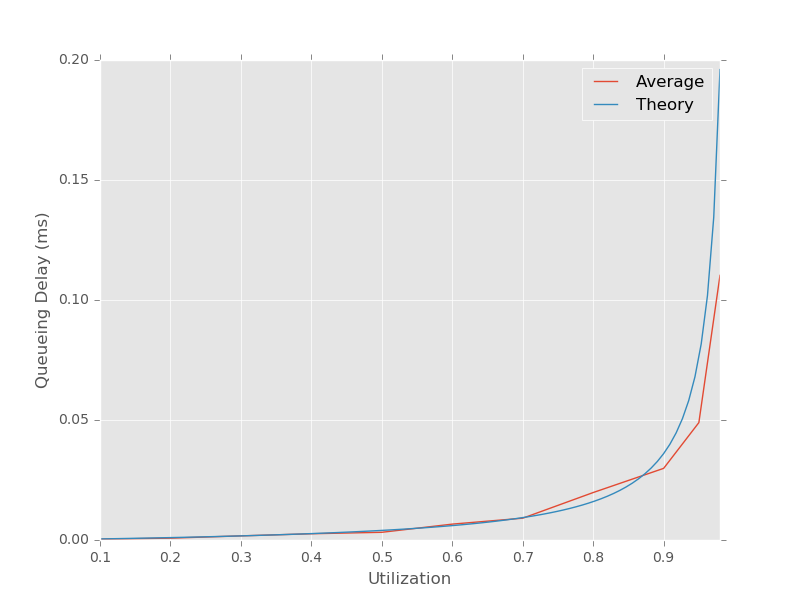
\includegraphics[width=15cm]{queing}
\end{figure}


Figure \ref{exp3fig} shows that the queueing delay results generated by our network closely match the theoretical queueing function. The slight varition between our results and the theoretical line might be due to the following factors:

\begin{itemize}
\item The packets used in our experiment were generated with some degree of randomness. While the theoretical equation uses probabilities to account for varying arrival times, the results of any given scenario will have some variation in general.
\item Our experiments were spaced out at utilization values of as much as 0.1. The plot of the data is therefore less smooth than the theoretical line. If more experiments were run with more utilization values and less gap between those values, the average results might more closely resemble the theoretical line.
\end{itemize}

\end{document}
